\documentclass[11pt,openany]{book}
\usepackage[]{graphicx}\usepackage[]{color}
%% maxwidth is the original width if it is less than linewidth
%% otherwise use linewidth (to make sure the graphics do not exceed the margin)
\makeatletter
\def\maxwidth{ %
  \ifdim\Gin@nat@width>\linewidth
    \linewidth
  \else
    \Gin@nat@width
  \fi
}
\makeatother

\definecolor{fgcolor}{rgb}{0.345, 0.345, 0.345}
\newcommand{\hlnum}[1]{\textcolor[rgb]{0.686,0.059,0.569}{#1}}%
\newcommand{\hlstr}[1]{\textcolor[rgb]{0.192,0.494,0.8}{#1}}%
\newcommand{\hlcom}[1]{\textcolor[rgb]{0.678,0.584,0.686}{\textit{#1}}}%
\newcommand{\hlopt}[1]{\textcolor[rgb]{0,0,0}{#1}}%
\newcommand{\hlstd}[1]{\textcolor[rgb]{0.345,0.345,0.345}{#1}}%
\newcommand{\hlkwa}[1]{\textcolor[rgb]{0.161,0.373,0.58}{\textbf{#1}}}%
\newcommand{\hlkwb}[1]{\textcolor[rgb]{0.69,0.353,0.396}{#1}}%
\newcommand{\hlkwc}[1]{\textcolor[rgb]{0.333,0.667,0.333}{#1}}%
\newcommand{\hlkwd}[1]{\textcolor[rgb]{0.737,0.353,0.396}{\textbf{#1}}}%
\let\hlipl\hlkwb

\usepackage{framed}
\makeatletter
\newenvironment{kframe}{%
 \def\at@end@of@kframe{}%
 \ifinner\ifhmode%
  \def\at@end@of@kframe{\end{minipage}}%
  \begin{minipage}{\columnwidth}%
 \fi\fi%
 \def\FrameCommand##1{\hskip\@totalleftmargin \hskip-\fboxsep
 \colorbox{shadecolor}{##1}\hskip-\fboxsep
     % There is no \\@totalrightmargin, so:
     \hskip-\linewidth \hskip-\@totalleftmargin \hskip\columnwidth}%
 \MakeFramed {\advance\hsize-\width
   \@totalleftmargin\z@ \linewidth\hsize
   \@setminipage}}%
 {\par\unskip\endMakeFramed%
 \at@end@of@kframe}
\makeatother

\definecolor{shadecolor}{rgb}{.97, .97, .97}
\definecolor{messagecolor}{rgb}{0, 0, 0}
\definecolor{warningcolor}{rgb}{1, 0, 1}
\definecolor{errorcolor}{rgb}{1, 0, 0}
\newenvironment{knitrout}{}{} % an empty environment to be redefined in TeX

\usepackage{alltt}
\newcommand{\SweaveOpts}[1]{}  % do not interfere with LaTeX
\newcommand{\SweaveInput}[1]{} % because they are not real TeX commands
\newcommand{\Sexpr}[1]{}       % will only be parsed by R


\usepackage[utf8]{inputenc} 
\usepackage{amssymb, amsmath, amsthm}
\usepackage{fullpage}
\usepackage{setspace}
\usepackage{graphicx}
\usepackage{natbib}
\usepackage{rotating}
\usepackage{caption}
\usepackage{subcaption}
\usepackage{multirow}
\usepackage{booktabs}
\usepackage{dcolumn}
\usepackage[grey]{quotchap}
\usepackage{xcolor}
\usepackage[left=1in, top=1in, right=1.5in, bottom=1in, headsep=.5in]
{geometry}
\usepackage{fancyhdr, blindtext}
\usepackage{diagbox}
\usepackage{hyperref} 
\usepackage{placeins}
\renewenvironment{knitrout}{\begin{singlespace}}{\end{singlespace}}
\newcommand*{\mybox}[2]{\colorbox{#1!30}{\parbox{.98\linewidth}{#2}}}
\newcommand*{\befehl}[1]{\texttt{\textbackslash #1}} % Added by 


\fancyhf{}
\fancyhead[LE]{\slshape \rightmark} 
\fancyhead[RE]{\thepage}
\fancyhead[RO]{\slshape \leftmark} 
\fancyhead[LO]{\thepage}
\renewcommand{\headrulewidth}{0.4pt}
\pagestyle{fancy}
%% new command for greybox
\long\def\greybox#1{%
    \newbox\contentbox%
    \newbox\bkgdbox%
    \setbox\contentbox\hbox to \hsize{%
        \vtop{
            \kern\columnsep
            \hbox to \hsize{%
                \kern\columnsep%
                \advance\hsize by -2\columnsep%
                \setlength{\textwidth}{\hsize}%
                \vbox{
                    \parskip=\baselineskip
                    \parindent=0bp
                    #1
                }%
                \kern\columnsep%
            }%
            \kern\columnsep%
        }%
    }%
    \setbox\bkgdbox\vbox{
        \pdfliteral{0.85 0.85 0.85 rg}
        \hrule width  \wd\contentbox %
               height \ht\contentbox %
               depth  \dp\contentbox
        \pdfliteral{0 0 0 rg}
    }%
    \wd\bkgdbox=0bp%
    \vbox{\hbox to \hsize{\box\bkgdbox\box\contentbox}}%
    \vskip\baselineskip%
}
%% make greybox (grbox) a float
\usepackage{float}
\newfloat{grbox}{thp}{lop}[section]
\floatname{grbox}{Grey Box}



\begin{document}





\chapter{Multiple Regression and Model Building} 

This book focuses on the use of systematic quantitative analysis for purposes of building, refining and testing theoretical propositions in the policy and social sciences. All of the tools discussed so far -- including univariate, bi-variate, and simple regression analysis -- provide means to evaluate distributions and test hypotheses concerning simple relationships. Most policy and social theories,  however, include multiple explanatory variables. \textit{Multiple regression} extends the utility of simple regression by permitting the inclusion of two or more explanatory variables.  This chapter discusses strategies for determining what variables to include (or exclude) in the model.  As before, we use the \texttt{tbur} data.  

\section{Model Building}

Model building is the process of deciding which independent variables to include in the model.\footnote{Model building also concerns decisions about model functional form, which we address in the next chapter.} For our purposes, when deciding which variables to include, theory and findings from the extant literature should be the most prominent guides. Apart from theory, however, this chapter examines empirical strategies that can help determine if the addition of new variables improves overall model fit. In general, when adding a variable check for: a) improved prediction based on empirical indicators, b) statistically and substantively significant estimated coefficients, and c) stability of model coefficients---do other coefficients change when adding the new one -- particularly look for sign changes.  

\subsection{Theory and Hypotheses}

The most important guidance for deciding whether a variable (or variables) should be included in your model is provided by theory and prior research. Simply put, knowing the literature on your topic is vital to knowing what variables are important. You should be able to articulate a clear theoretical reason for including each variable in your model. In those cases where you don't have much theoretical guidance, however, you should use model \textit{parsimony}, which is a function of simplicity and model fit, as your guide. You can focus on whether the inclusion of a variable improves model fit.  In the next section, we will explore several empirical indicators that can be used to evaluate the appropriateness of inclusion of variables. 

\subsection{Empirical Indicators}

When building a model, it is best to start with a few IV's and then begin adding other variables. However, when adding a variable, check for: 
\begin{enumerate}
\item Improved prediction (increase in adjusted $R^2$)
\item Statistically and substantively significant estimated coefficients
\item Stability of model coefficients
  \begin{itemize}
\item Do other coefficients change when adding the new one?
\item Particularly look for sign changes for estimated coefficients.
  \end{itemize}
  \end{enumerate}

\subsubsection{Coefficient of Determination: $R^2$}

$R^2$ was previously discussed within the context of simple regression. The extension to multiple regression is straightforward, except that multiple regression leads us to place greater weight on the use of the \textbf{adjusted $R^2$}. Recall that the adjusted $R^2$ corrects for the inclusion of multiple independent variables; $R^{2}$ is the ratio of the explained sum of squares to the total sum of squares (\textit{ESS/TSS}). The components of $R^{2}$ for an observation are illustrated in Figure \ref{fig:rsq}. As before, for each observation $Y_{i}$, variation around the mean can be decomposed into that which is ``explained" by the regression model and that which is not.  
\begin{figure}
  \centering
  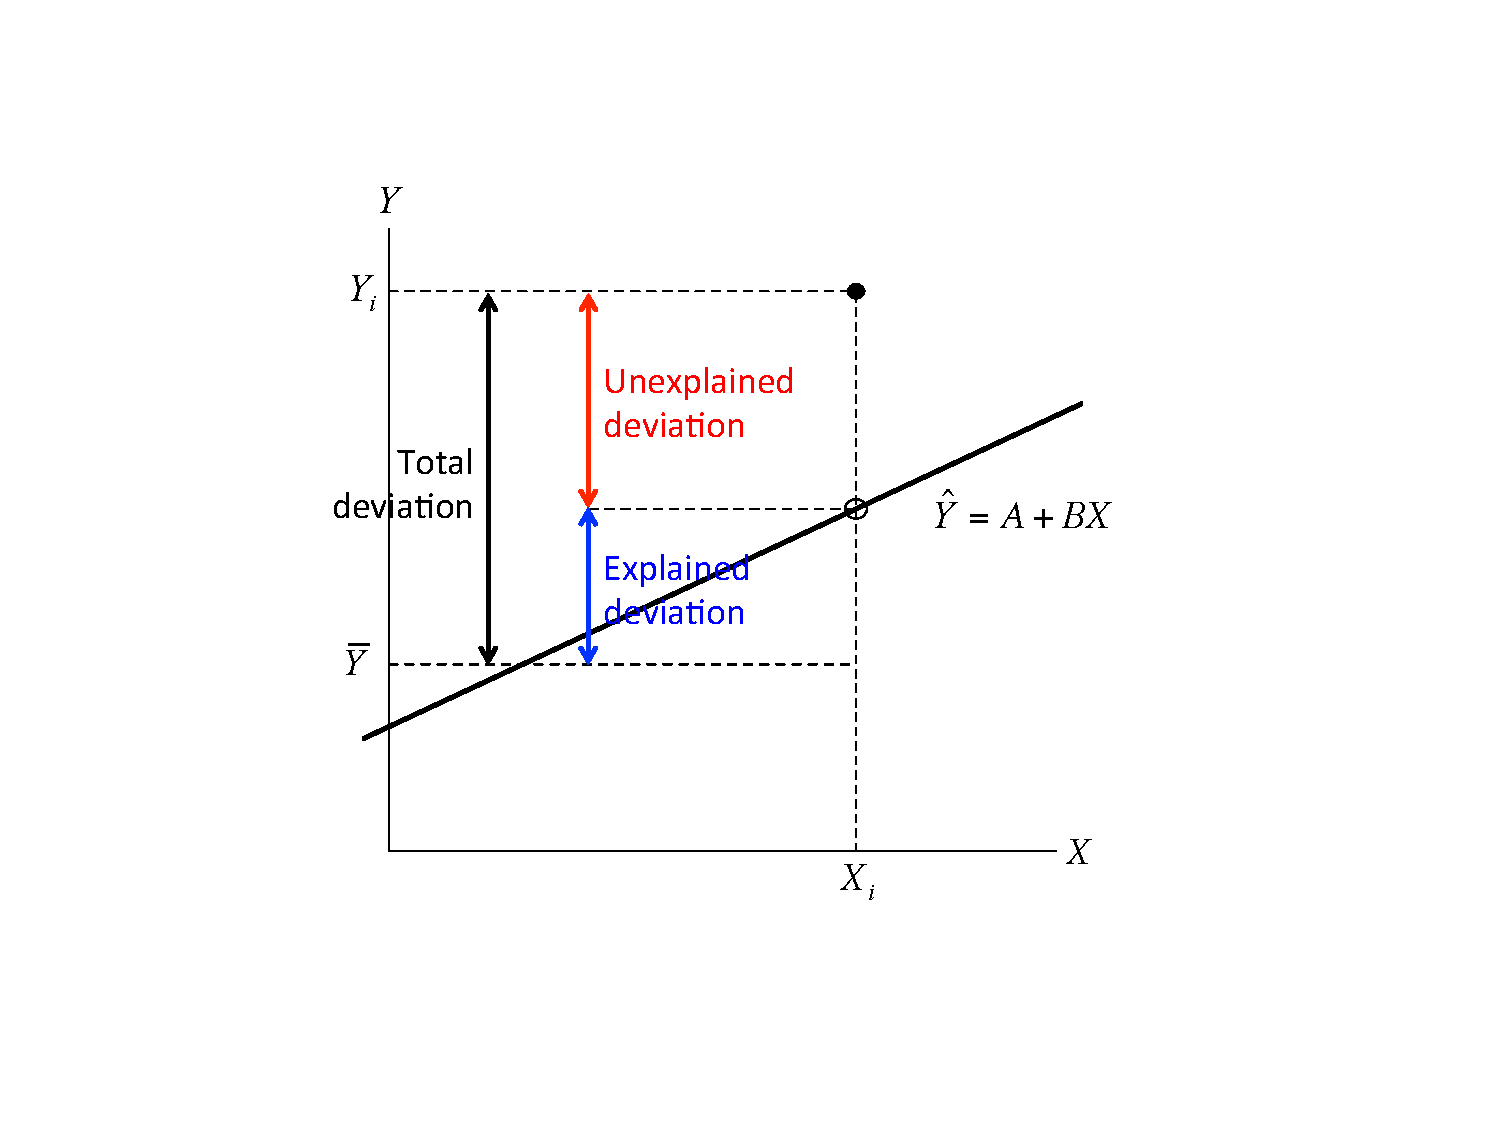
\includegraphics[width=5in]{../13_ModelFit/rsquared.pdf}
  \caption[$R^{2}$]{ \label{fig:rsq}}
\end{figure}

$R^2$ is expressed as: 
\begin{equation}
 R^{2} = 1-\frac{RSS}{TSS}  
\end{equation}

However, this formulation of $R^2$ is insensitive to the complexity of the model and the degrees of freedom provided by your data. This means that an increase in the number of $k$ independent variables, can increase the $R^2$. Adjusted $R^2$ penalizes the $R^2$ by correcting for the degrees of freedom. It is defined as: 
\begin{equation}
 \text{adjusted} R^2 = 1-\frac{\frac{RSS}{n-k-1}}{\frac{TSS}{n-k-1}}
\end{equation}

The $R^2$ of two models can be compared, as illustrated by the following example. The first (simpler) model consists of basic demographics (age, education, and income) as predictors of climate change risk. The second (more complex) model adds the variable measuring political ideology to the explanation.


\begin{knitrout}
\definecolor{shadecolor}{rgb}{0.969, 0.969, 0.969}\color{fgcolor}\begin{kframe}
\begin{alltt}
\hlstd{ds.temp} \hlkwb{<-} \hlkwd{filter}\hlstd{(ds)} \hlopt
  \hlkwd{select}\hlstd{(glbcc_risk, age, education, income, ideol)} \hlopt
  \hlkwd{na.omit}\hlstd{()}

\hlstd{ols1} \hlkwb{<-} \hlkwd{lm}\hlstd{(glbcc_risk} \hlopt{~} \hlstd{age} \hlopt{+} \hlstd{education} \hlopt{+} \hlstd{income,} \hlkwc{data} \hlstd{= ds.temp)}
\hlkwd{summary}\hlstd{(ols1)}
\end{alltt}
\begin{verbatim}
## 
## Call:
## lm(formula = glbcc_risk ~ age + education + income, data = ds.temp)
## 
## Residuals:
##     Min      1Q  Median      3Q     Max 
## -6.9189 -2.0546  0.0828  2.5823  5.1908 
## 
## Coefficients:
##               Estimate Std. Error t value Pr(>|t|)    
## (Intercept)  6.161e+00  3.425e-01  17.987  < 2e-16 ***
## age         -1.557e-02  4.519e-03  -3.446  0.00058 ***
## education    2.253e-01  3.657e-02   6.160 8.58e-10 ***
## income      -5.576e-06  1.110e-06  -5.022 5.51e-07 ***
## ---
## Signif. codes:  0 '***' 0.001 '**' 0.01 '*' 0.05 '.' 0.1 ' ' 1
## 
## Residual standard error: 3.008 on 2268 degrees of freedom
## Multiple R-squared:  0.02565,	Adjusted R-squared:  0.02437 
## F-statistic: 19.91 on 3 and 2268 DF,  p-value: 9.815e-13
\end{verbatim}
\begin{alltt}
\hlstd{ols2} \hlkwb{<-} \hlkwd{lm}\hlstd{(glbcc_risk} \hlopt{~} \hlstd{age} \hlopt{+} \hlstd{education} \hlopt{+} \hlstd{income} \hlopt{+} \hlstd{ideol,} \hlkwc{data} \hlstd{= ds.temp)}
\hlkwd{summary}\hlstd{(ols2)}
\end{alltt}
\begin{verbatim}
## 
## Call:
## lm(formula = glbcc_risk ~ age + education + income + ideol, data = ds.temp)
## 
## Residuals:
##     Min      1Q  Median      3Q     Max 
## -8.7991 -1.6654  0.2246  1.4437  6.5968 
## 
## Coefficients:
##               Estimate Std. Error t value Pr(>|t|)    
## (Intercept)  1.092e+01  3.092e-01  35.326  < 2e-16 ***
## age         -4.423e-03  3.669e-03  -1.206  0.22810    
## education    6.328e-02  2.994e-02   2.113  0.03468 *  
## income      -2.603e-06  9.021e-07  -2.886  0.00394 ** 
## ideol       -1.037e+00  2.992e-02 -34.650  < 2e-16 ***
## ---
## Signif. codes:  0 '***' 0.001 '**' 0.01 '*' 0.05 '.' 0.1 ' ' 1
## 
## Residual standard error: 2.433 on 2267 degrees of freedom
## Multiple R-squared:  0.363,	Adjusted R-squared:  0.3619 
## F-statistic:   323 on 4 and 2267 DF,  p-value: < 2.2e-16
\end{verbatim}
\end{kframe}
\end{knitrout}
As can be seen by comparing the model results, the more complex model that includes political ideology has a higher $R^2$ than does the simpler model. This indicates that the more complex model explains a greater fraction of the variance in perceived risks of climate change. However, we don't know if this improvement is statistically significant. In order to determine whether the more complex model adds significantly to the explanation of perceive risks, we can utilize the $F$-test.  

\subsubsection{$F$-test}

The $F$-test is a test statistic based on the $F$ distribution, in the same way the the $t$-test is based on the $t$ distribution. The $F$ distribution skews right and ranges between $0$ and $\infty$. Just like the $t$ distribution, the $F$ distribution approaches normal as the degrees of freedom increase.\footnote{Note that the $F$ distribution is the square of a $t$-distributed variable with $m$ degrees of freedom. The $F$ distribution has $1$ degree of freedom in the numerator and $m$ degrees of in the denominator: 
\begin{equation*}
  t^2_m = F_{1,m} 
\end{equation*}}

$F$-tests are used to test for the statistical significance of the overall model fit. The null hypothesis for an $F$-test is that the model offers no improvement for predicting $Y_i$ over the mean of $Y$,
$\bar{Y}$. 

The formula for the $F$-test is: 

\begin{equation}
  F = \frac{\frac{ESS}{k}}{\frac{RSS}{n-k-1}}
\end{equation}

\noindent where $k$ is the number of parameters and $n-k-1$ are the degrees of freedom. Therefore, $F$ is a ratio of the explained variance to the residual variance, correcting for the number of observations and parameters. The $F$-value is compared to the $F$-distribution, just like a $t$-distribution, to obtain a $p$-value. Note that the \texttt{R} output includes the $F$ statistic and $p$ value. 

\subsubsection{Nested $F$-test}

For model building we turn to the nested $F$-test, which tests whether a more complex model (with more IVs) adds to the explanatory power over a simpler model (with fewer IVs). To find out, we calculate an F-statistic for the model improvement: 

\begin{equation}
  F = \frac{\frac{ESS_1-ESS_0}{q}}{\frac{RSS_1}{n-k-1}}
\end{equation}

\noindent where $q$ is the difference in the number of IVs between the simpler and the mode complex models.  The complex model has $k$ IVs (and estimates $k$ parameters), and the simpler model has $k-q$ IVs (and estimates only $k-q$ parameters). $ESS_1$ is the explained sum of squares
for the complex model. $RSS_1$ is the residual sum of squares for the complex model. $ESS_0$ is the explained sum of squares for the simpler
model. So the nested-F represents the ratio of the additional explanation per added IV, over the residual sum of squares divided by the model degrees of freedom.

We can use \texttt{R}, to calculate the $F$ statistic based on our previous example.  
\begin{knitrout}
\definecolor{shadecolor}{rgb}{0.969, 0.969, 0.969}\color{fgcolor}\begin{kframe}
\begin{alltt}
\hlstd{TSS} \hlkwb{<-} \hlkwd{sum}\hlstd{((ds.temp}\hlopt{$}\hlstd{glbcc_risk}\hlopt{-}\hlkwd{mean}\hlstd{(ds.temp}\hlopt{$}\hlstd{glbcc_risk))}\hlopt{^}\hlnum{2}\hlstd{)}
\hlstd{TSS}
\end{alltt}
\begin{verbatim}
## [1] 21059.86
\end{verbatim}
\begin{alltt}
\hlstd{RSS.mod1} \hlkwb{<-} \hlkwd{sum}\hlstd{(ols1}\hlopt{$}\hlstd{residuals}\hlopt{^}\hlnum{2}\hlstd{)}
\hlstd{RSS.mod1}
\end{alltt}
\begin{verbatim}
## [1] 20519.57
\end{verbatim}
\begin{alltt}
\hlstd{ESS.mod1} \hlkwb{<-} \hlstd{TSS}\hlopt{-}\hlstd{RSS.mod1}
\hlstd{ESS.mod1}
\end{alltt}
\begin{verbatim}
## [1] 540.2891
\end{verbatim}
\begin{alltt}
\hlstd{RSS.mod2} \hlkwb{<-} \hlkwd{sum}\hlstd{(ols2}\hlopt{$}\hlstd{residuals}\hlopt{^}\hlnum{2}\hlstd{)}
\hlstd{RSS.mod2}
\end{alltt}
\begin{verbatim}
## [1] 13414.89
\end{verbatim}
\begin{alltt}
\hlstd{ESS.mod2} \hlkwb{<-} \hlstd{TSS}\hlopt{-}\hlstd{RSS.mod2}
\hlstd{ESS.mod2}
\end{alltt}
\begin{verbatim}
## [1] 7644.965
\end{verbatim}
\begin{alltt}
\hlstd{F} \hlkwb{<-} \hlstd{((ESS.mod2} \hlopt{-} \hlstd{ESS.mod1)}\hlopt{/}\hlnum{1}\hlstd{)}\hlopt{/}\hlstd{(RSS.mod2}\hlopt{/}\hlstd{(}\hlkwd{length}\hlstd{(ds.temp}\hlopt{$}\hlstd{glbcc_risk)}\hlopt{-}\hlnum{4}\hlopt{-}\hlnum{1}\hlstd{))}
\hlstd{F}
\end{alltt}
\begin{verbatim}
## [1] 1200.629
\end{verbatim}
\end{kframe}
\end{knitrout}
Or, you can simply use the \texttt{anova} function in $R$: 
\begin{knitrout}
\definecolor{shadecolor}{rgb}{0.969, 0.969, 0.969}\color{fgcolor}\begin{kframe}
\begin{alltt}
\hlkwd{anova}\hlstd{(ols1,ols2)}
\end{alltt}
\begin{verbatim}
## Analysis of Variance Table
## 
## Model 1: glbcc_risk ~ age + education + income
## Model 2: glbcc_risk ~ age + education + income + ideol
##   Res.Df   RSS Df Sum of Sq      F    Pr(>F)    
## 1   2268 20520                                  
## 2   2267 13415  1    7104.7 1200.6 < 2.2e-16 ***
## ---
## Signif. codes:  0 '***' 0.001 '**' 0.01 '*' 0.05 '.' 0.1 ' ' 1
\end{verbatim}
\end{kframe}
\end{knitrout}

\noindent As shown using both approaches, the inclusion of ideology significantly improves model fit. 

\subsection{Risks in Model Building}

As is true of most things in life, there are risks to consider when building statistical models. First, are you including irrelevant $X$'s? These can increase model complexity, reduce adjusted $R^2$, and  increase model variability across samples. Remember that you should have a theoretical basis for inclusion of all of the variables in your model. 

Second, are you omitting relevant $X$'s? Not including important variables can fail to capture fit and can bias other estimated coefficients, particularly when the omitted $X$ is related to both other $X$'s and to the dependent variable $Y$. 

Finally, remember that we are using sample data. Therefore, about 5\% of the time, our sample will include random observations of $X$'s that result in $B$'s that meet classical hypothesis tests -- resulting in a Type I error. Conversely, the $B$'s may be important, but the sample data will randomly include observations of $X$ that result in estimated parameters that do not meet  the classical statistical tests -- resulting in a Type II error.  That's why we rely on theory, prior hypotheses, and replication. 

\section{Evils of Stepwise Regression}

Almost all statistical software packages (including $R$) permit a number of mechanical ``search strategies" for finding IVs that make a statistically significant contribution to the prediction of the model dependent variable. The most common of these is called \texttt{stepwise regression}, which may also be referred to as forward, backward (or maybe even upside down!) stepwise regression. Stepwise procedures do not require that the analyst think -- you just have to designate a pool of possible IVs and let the package go to work, sifting through the IVs to identify those that (on the
basis of your sample data) appear to be related to the model dependent variable.  The stepwise procedures use sequential F-tests, sequentially adding variables that ``improve the fit" of the mindless model until there are no more IVs that meet some threshold (usually $p<0.05$) of statistical significance. These procedures are like mechanically wringing all of the explanation you can get for $Y$ out of some pool of $X$.

You should already recognize that these kind of methods pose serious problems. First and foremost, this is an atheoretical approach to model building. But, what if you have no theory to start with -- is a stepwise approach appropriate then? No, for several reasons. If any of the candidate $X$ variables are strongly correlated, the inclusion of the first one will ``use up" some of the explanation of the second, because of the way OLS calculates partial regression coefficients. For that reason, once one of the variables is mechanically selected, the other will tend to be excluded because it will have less to contribute to $Y$. Perhaps more damning, stepwise approaches as highly susceptible to inclusion of spuriously related variables. Recall that we are using samples, drawn from the larger population, and that samples are subject to random variation. If the step-wise process uses the classical 0.05 cut-off for inclusion of a variable, that means that one time in twenty (in the long run) we will include a variable that meets the criterion only by random chance.\footnote{Add to that the propensity of journals to publish articles that have new and exciting findings, in the form of statistically significant modeled coefficients, and you can see that there would be a substantial risk: that of finding and promoting nonsense findings.} Recall that the classical hypothesis test requires that we specify our hypothesis in advance; step-wise processes simply rummage around within a set of potential IVs to find those that fit.

There have been notable cases in which mechanical model building has resulted in seriously problematic ``findings" that have very costly implications for society. One is recounted in the PBS Frontline episode called ``Currents of Fear".\footnote{The program was written, produced  and directed by Jon Palfreman, and it was first broadcast on June 13, 1995. The full transcript can be found here: http://www.pbs.org/wgbh/pages/frontline/programs/transcripts/1319.html} The story concerns whether electromagnetic fields (EMFs) from technologies including high-voltage power lines cause cancer in people who are exposed. The problem was that ``cancer clusters" could be identified that were proximate to the power lines, but no laboratory experiments could find a connection. But concerned citizens and activists persisted in believing there was a causal relationship. In that context, the Swedish government sponsored a very ambitious study to settle the question. Here is the text of the discussion from  the Frontline program:

\begin{quote}
... in 1992, a landmark study appeared from Sweden. A huge investigation, it enrolled everyone  living within 300 meters of Sweden's high-voltage  transmission line system over a 25-year period.  They went far beyond all previous studies in their efforts to measure magnetic fields, calculating the fields that the children were exposed to at the time of their cancer diagnosis and before. This study  reported an apparently clear association between magnetic field exposure and childhood leukemia, with a risk ratio for the most highly exposed of nearly 4.

The Swedish government announced it was investigating new policy options, including whether to  move children away from schools near power lines. Surely, here was the proof that power lines were  dangerous, the proof that even the physicists and biological naysayers would have to accept. But three years after the study was published, the Swedish research no longer looks so unassailable. This is a  copy of the original contractor's report, which reveals the remarkable thoroughness of the Swedish team.  Unlike the published article, which just summarizes part of the data, the report shows everything they did in  great detail, all the things they measured and all the comparisons they made.

When scientists saw how many things they had measured -- nearly 800 risk ratios are in the report -- they began accusing the Swedes of falling into one of the most fundamental errors in epidemiology, sometimes called the multiple comparisons fallacy.
\end{quote}

So, according to the Frontline report, the Swedish EMF study regressed the incidence of nearly  800 possible cancers onto the proximity of its citizens to high-voltage power lines. In some cases, there appeared to be a positive relationship. These they reported. In other cases, there was no relationship, and in some the relationship was negative - which would seem to imply (if you were so silly as to do so) that living near the high voltage lines actually protected people from cancer. But only the positive relationships were included in the reports, leading to a false impression that the study had confirmed that proximity to high-voltage lines causes cancer. Embarrassing to the study authors, to put it mildly.

\section{Summary}

This chapter has focused on multiple regression model building. The keys to that process are understanding (a) the critical role of theory and prior research findings in model specification, and (b) the meaning of the partial regression coefficients produced by OLS. When theory is not well-developed, you can thoughtfully employ nested F-tests to evaluate whether the hypothesized inclusion of an $X$ variable meaningfully contributes to the explanation of $Y$. But you should avoid reliance on mechanical model-building routines, like step-wise regression, because these can lead you down into statistical perdition. None of us want to see that happen!


\end{document}
